\documentclass[a4paper,11pt]{scrartcl}
\usepackage[bookmarks,pagebackref,colorlinks=true,linkcolor=blue,urlcolor=blue,citecolor=blue]{hyperref}
\usepackage[utf8]{inputenc}
\usepackage{amssymb}
\usepackage{amsmath}
\usepackage{tikz}
\usepackage{tikz-cd}
\usetikzlibrary{3d}
\usepackage{tikz-3dplot}
\usepackage{pgfplots}
\usepackage[colorinlistoftodos]{todonotes}
\usepackage{color}
\pgfplotsset{compat=1.16}

\begin{document}

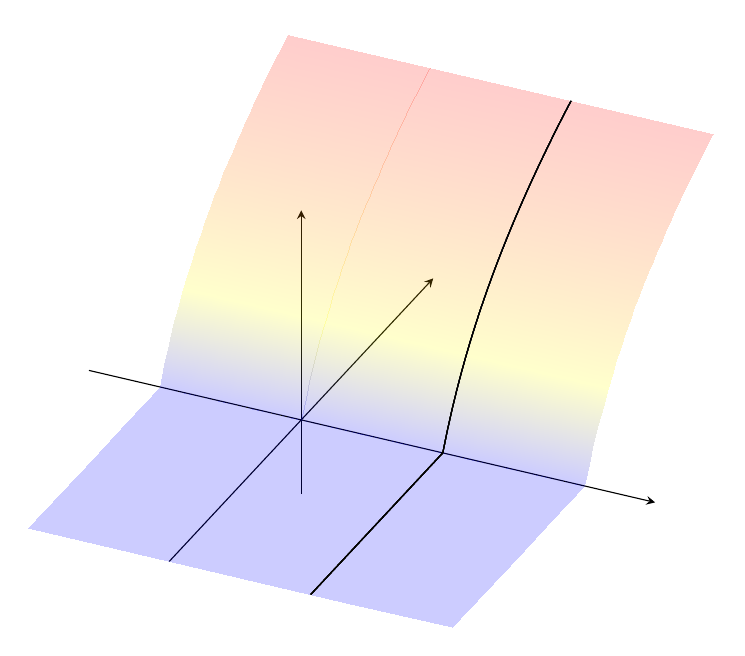
\begin{tikzpicture}
    \begin{axis}[width=\textwidth,
    axis equal,
    xmin=-1,xmax=2,ymin=-2,ymax=2,zmin=0,zmax=1,
    xtick=\empty,ytick=\empty, ztick=\empty,
    axis lines=center]

    \addplot3[surf, opacity=0.2, shader=interp, domain=-1:2,y domain=-2:0,samples=5]
    ({x}, {y}, {0});
    \addplot3[surf, opacity=0.2, shader=interp, domain=0:2,y domain=0:2,samples=30]
    ({x}, {y}, {ln(2*y+1)});
    \addplot3[surf, opacity=0.2, shader=interp, domain=-1:0,y domain=0:2,samples=30]
    ({x}, {y}, {ln(2*y+1)});
    \addplot3[mesh, draw=black,shader=interp, opacity=0.2,domain=-2:0,samples=30]
    ({1}, {x}, {0});
    \addplot3[mesh, draw=black,shader=interp, opacity=0.2,domain=0:2,samples=30]
    ({1}, {x}, {ln(2*x+1)});

    \end{axis}
\end{tikzpicture}

\end{document}